\documentclass{article}
\usepackage{graphicx} % Required for inserting images
\usepackage{amsmath}
\usepackage{geometry}
\usepackage{url}

\newgeometry{margin=1in, top=4cm}

\title{\textbf{Medical Physics Prerequisites}}
\author{Michelangelo Boscolo}
\date{June 2026}



\begin{document}

\maketitle
%\tableofcontents 

\begin{center}
    {\Large \textbf{Introduction}} \\
    \vspace{0.5cm}
    Hi, i made this recap for the prerequisites question of the medical physics exam. I've included the things that seem to me to be the most frequently asked. if you want to add something else you can go to the GitHub repository \\ \url{https://github.com/Michelangelo01/Medical-Physics-Prerequisites} \\
    (it's public) and edit the source code.
\end{center}

\vspace{3cm}

\section{Photon - matter interaction}

When a photon (a packet of light or X-ray/gamma-ray energy) passes through matter, it doesn't just pass through quietly. Depending on how much energy it’s packing, it will interact with the atoms it encounters in one of three major ways: the \textbf{Photoelectric Effect}, \textbf{Compton Scattering}, or \textbf{Pair Production}.  Here is a breakdown of how each process works, moving from the lowest energy to the highest energy.

\begin{enumerate}
    \item The Photoelectric Effect (Low Energy). In the photoelectric effect, a relatively low-energy photon collides with a tightly bound inner-shell electron of an atom. The photon transfers all of its energy to the electron and vanishes completely. If the photon's energy is greater than the binding energy holding the electron to the nucleus, the electron is ejected from the atom. This ejected electron is called a photoelectron. 
    \begin{figure}[h!]
        \centering
        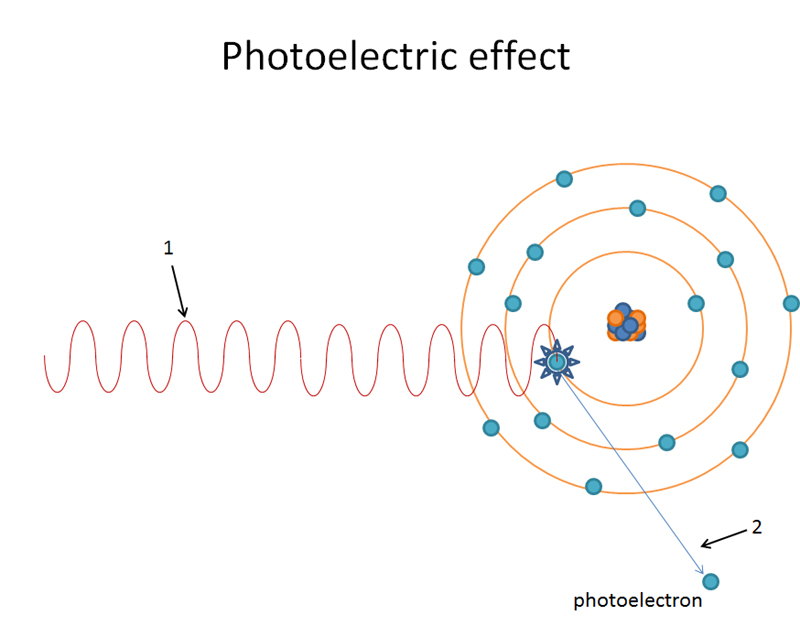
\includegraphics[scale=0.3]{Figures/photoelectric-effect-1.jpg}
        \caption{Photoelectric effect.}
        \label{1}
    \end{figure}
    Because a vacancy is left in the inner shell, a higher-shell electron drops down to fill the gap, releasing a characteristic X-ray photon in the process. The photon is completely absorbed. This is the dominant process at low energies and is highly dependent on the atomic number ($Z$) of the material (which is why lead is so great at shielding low-energy X-rays).

    \newpage
    \item 
    Compton Scattering (Medium Energy). As photon energy increases, the photon becomes too energetic to be completely absorbed by a bound electron. Instead, it undergoes Compton scattering, which is essentially a billiard-ball collision. The incoming high-energy photon collides with a loosely bound outer-shell electron. The photon transfers part of its energy to the electron. The electron is knocked out of the atom (called a Compton recoil electron), and the photon "bounces off" or scatters at an angle with less energy and a longer wavelength.  

    \begin{figure}[h!]
        \centering
        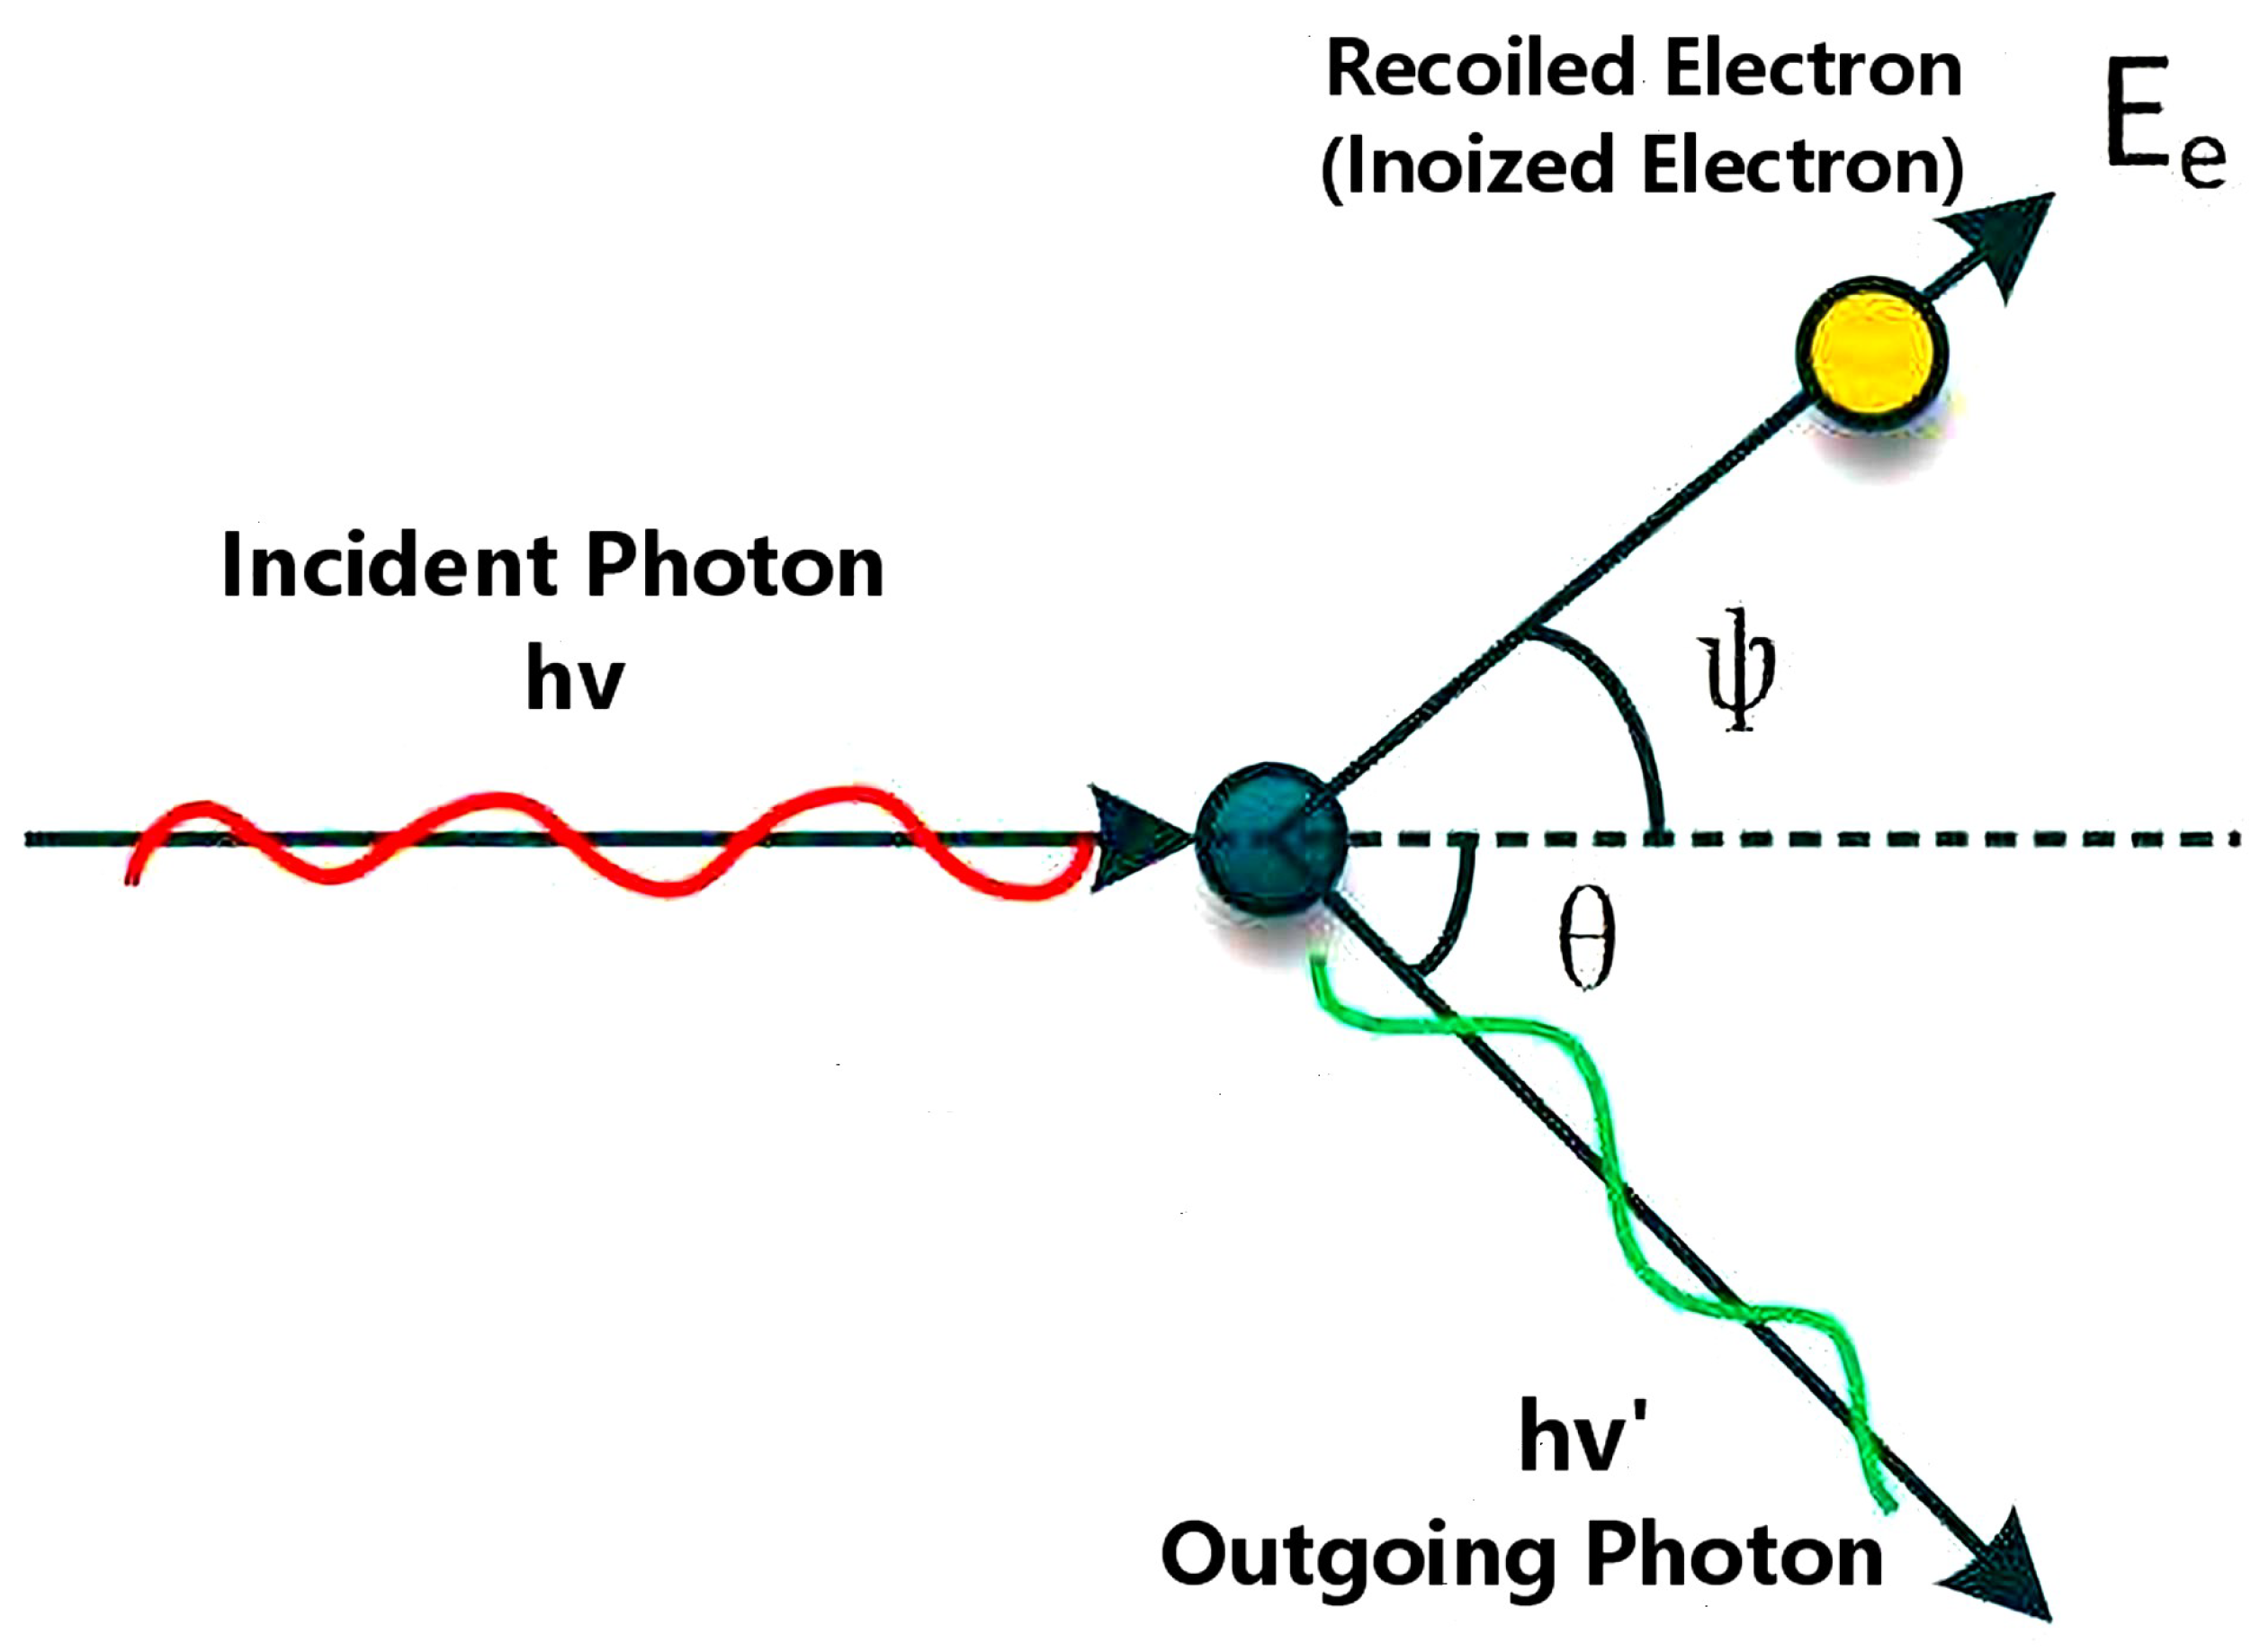
\includegraphics[scale=0.5]{Figures/compton scattering.png}
        \caption{Compton scattering.}
        \label{2}
    \end{figure}
    
    The energy of the scattered photon depends on the angle at which it scatters, described by the Compton scattering formula: 
    $$E' = \frac{E}{1 + \frac{E}{m_e c^2} (1 - \cos\theta)}$$
    The photon is not destroyed; it is just deflected and degraded in energy. This is the most common interaction in the energy ranges used for daily medical imaging (like diagnostic X-rays and radiation therapy).

    

    \item Pair Production (High Energy). When a photon has extremely high energy, it can interact directly with the intense electric field near the atomic nucleus. The photon completely disappears, and its pure energy is converted directly into mass, creating a pair of particles: an electron and a positron (the electron's antimatter twin). Because energy and mass are interchangeable ($E = mc^2$), the photon must have a minimum "threshold" energy equal to the rest mass of both particles. The rest mass of an electron (or positron) is $0.511 \text{ MeV}$. Therefore, pair production cannot happen unless the photon has at least $1.022 \text{ MeV}$ of energy.  The Aftermath: Any excess energy above $1.022 \text{ MeV}$ becomes kinetic energy, sending the electron and positron flying off. Eventually, the positron will slow down, meet another electron, and undergo annihilation, converting back into two photons.

    \begin{figure}[h!]
        \centering
        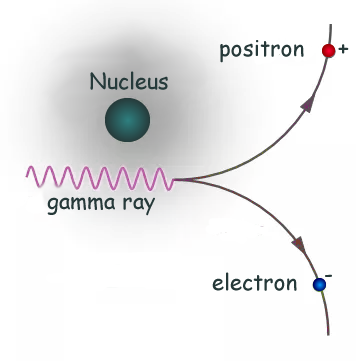
\includegraphics[scale=0.35]{Figures/pairproduction.png}
        \caption{Pair production.}
        \label{3}
    \end{figure}
\end{enumerate}

\begin{figure}[h!]
        \centering
        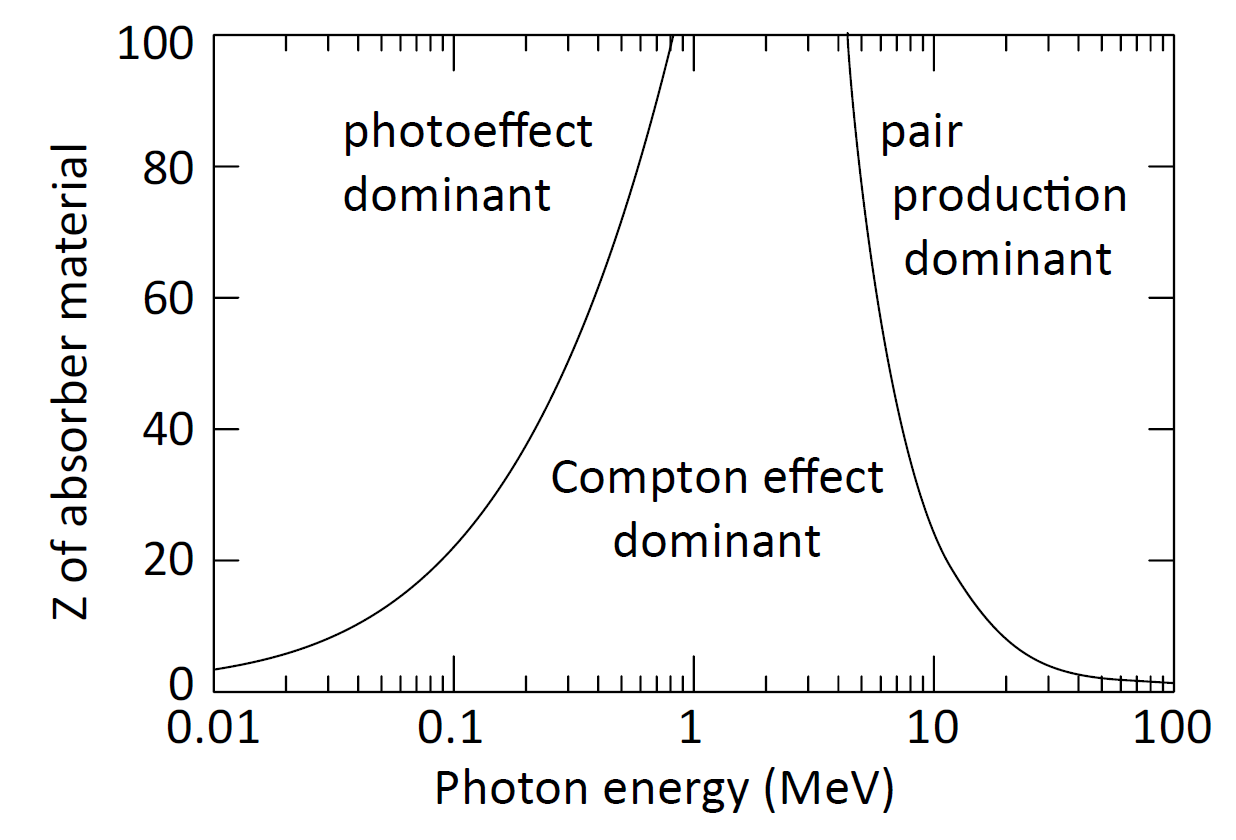
\includegraphics[scale=0.4]{Figures/int rad materia.png}
        \caption{regions of predominance of each effect.}
        \label{4}
    \end{figure}

When you shine a beam of light (or X-rays, or gamma rays) through a material, it doesn't all make it to the other side. Some of it gets absorbed, and some gets scattered. This reduction in the intensity of the beam is called photon attenuation. Especially when dealing with X-rays or radiation shielding, you'll often see the law expressed in terms of the beam's intensity ($I$): $$I = I_0 e^{-\mu x}$$ $I_0$ is the initial intensity of the photons, $I$ is the intensity after passing through the material, $\mu$ (mu) is the linear attenuation coefficient (how easily the material attenuates the photon beam) and $x$ is the thickness of the material. This exponential decay means that the first centimeter of a material blocks a much larger absolute number of photons than the second centimeter, but the percentage of remaining photons blocked per centimeter stays constant. 


\begin{figure}[h!]
        \centering
        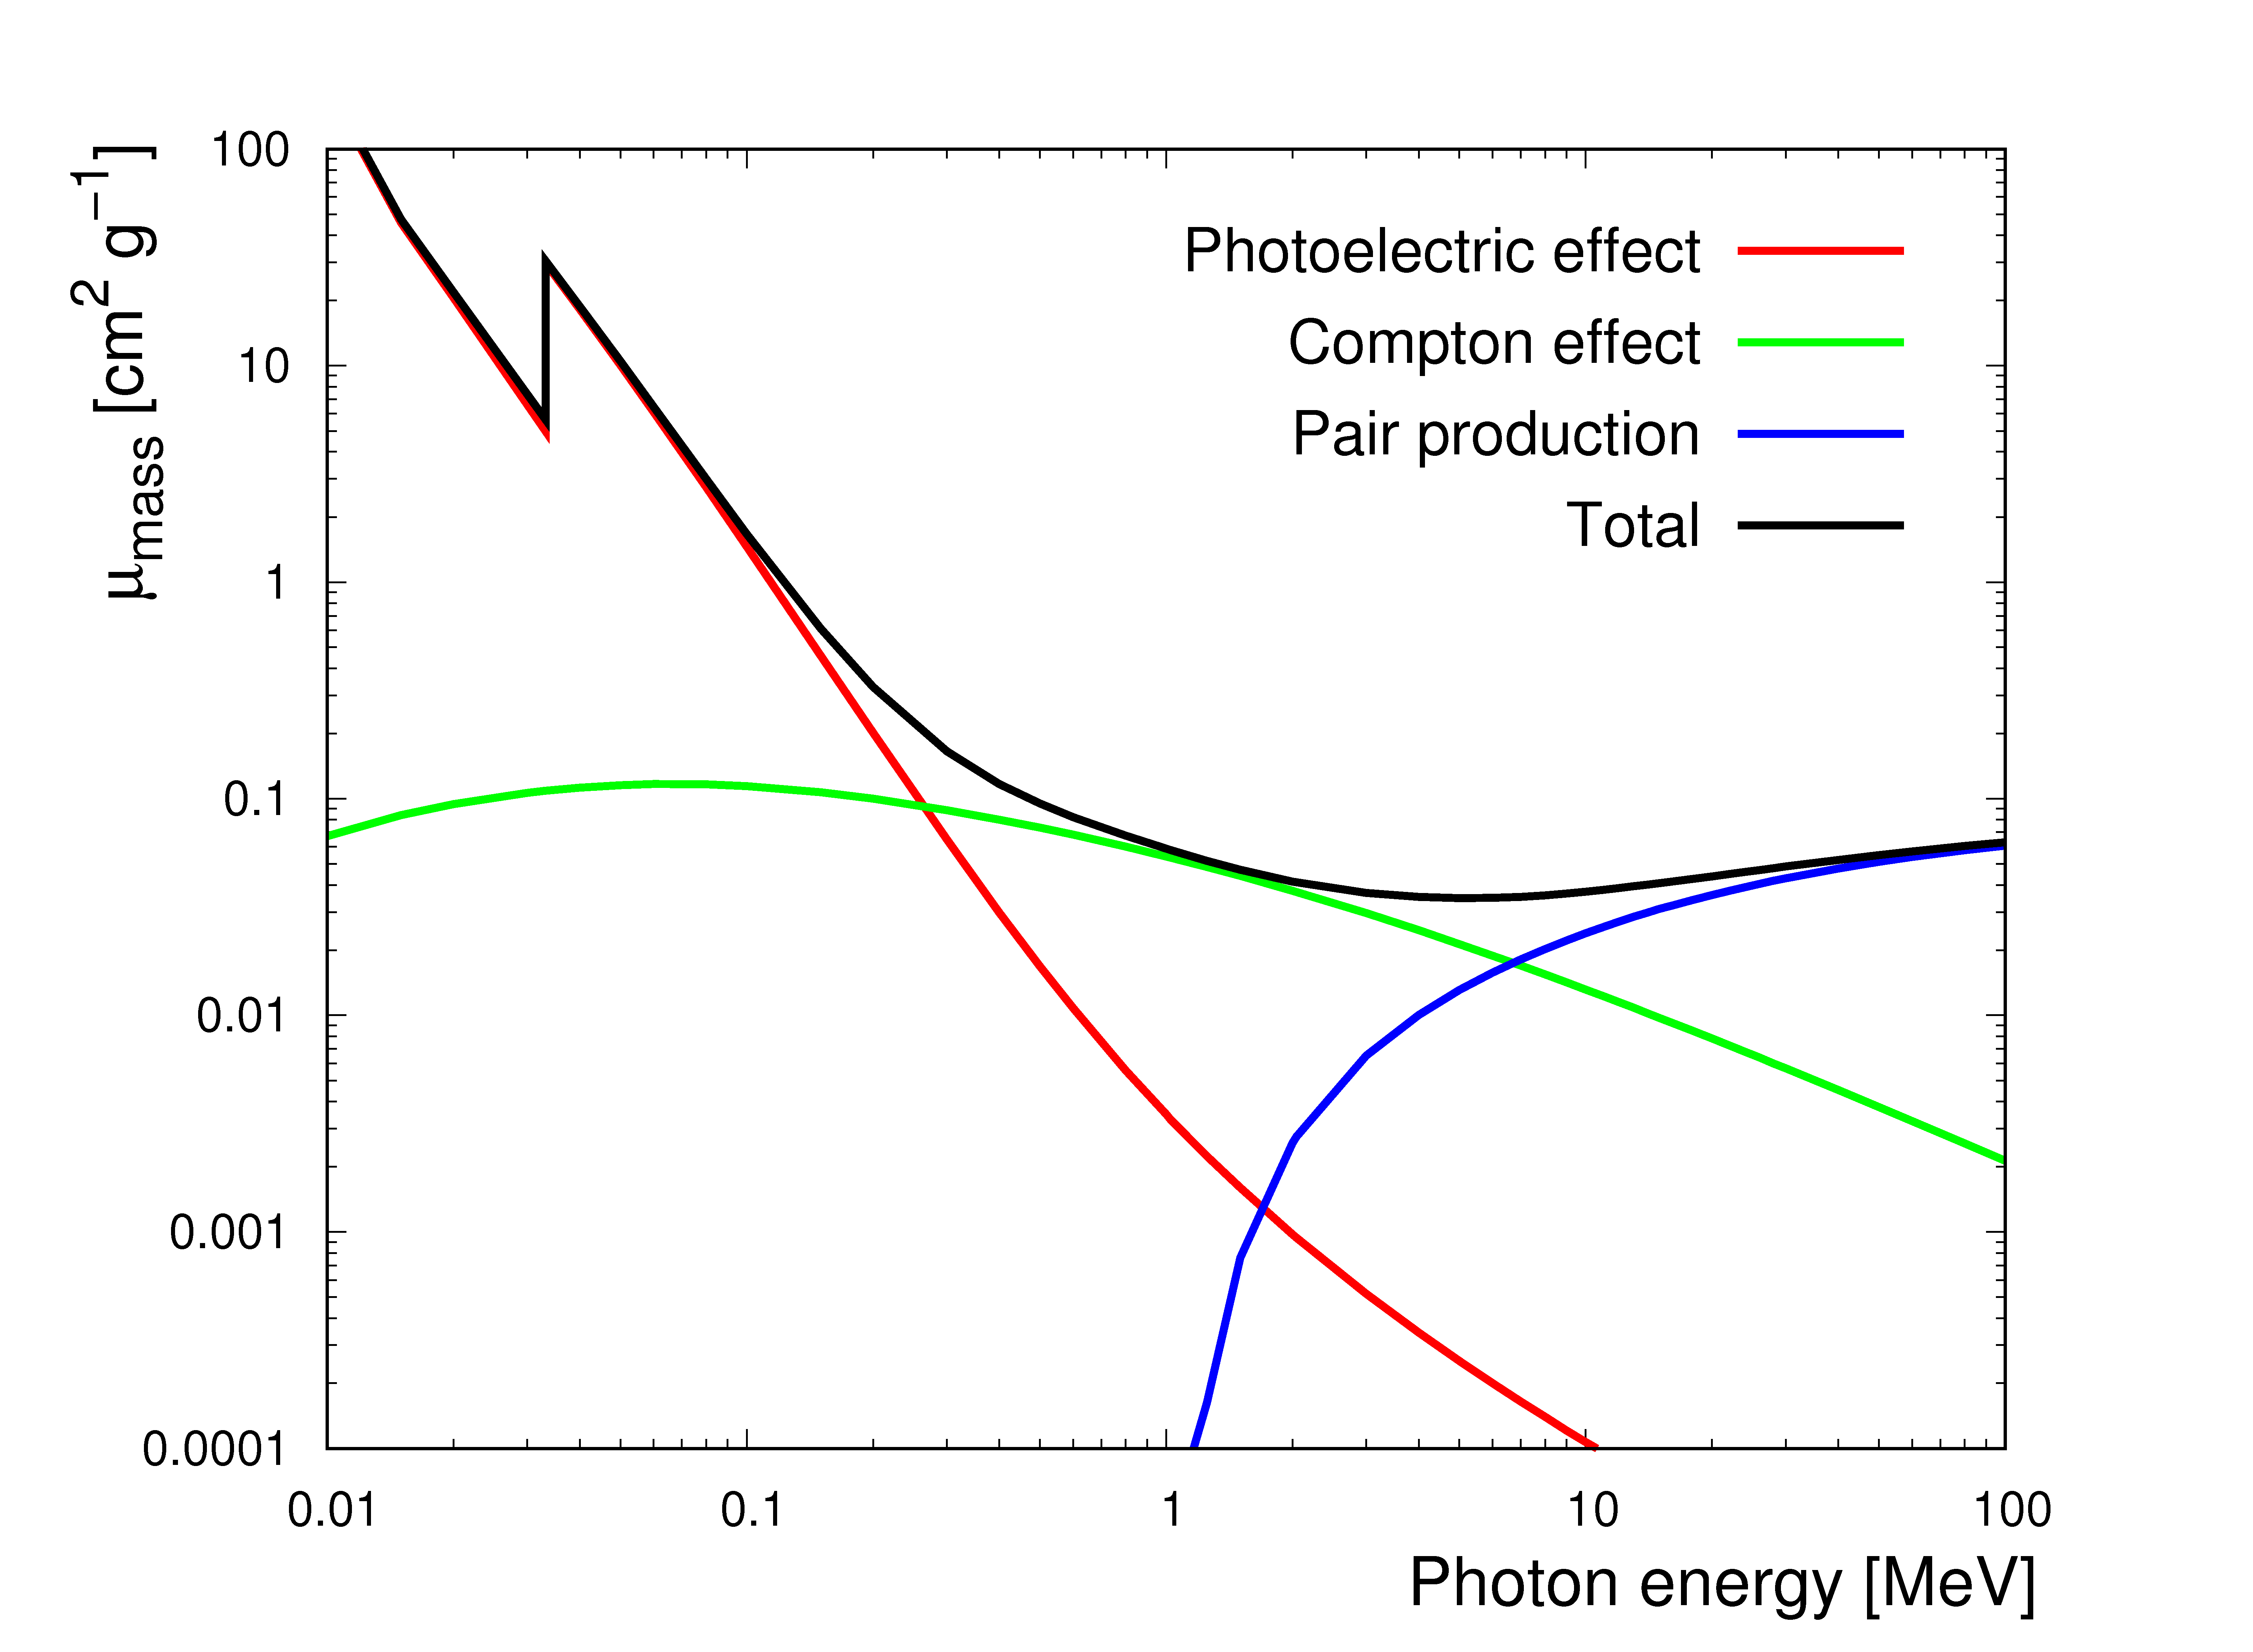
\includegraphics[scale=0.06]{Figures/attenuation photonsù.png}
        \caption{Attenuation coefficient with varying energy.}
        \label{5}
    \end{figure}


\section{Charged particle - matter interaction (stopping power)}

When a heavy charged particle (like a proton, alpha particle, or ion) traverses matter, it interacts primarily via the electromagnetic force with the atomic electrons of the medium. Because the particle is much heavier than an electron, it moves in a virtually straight line, losing energy in a continuous stream of tiny increments through thousands of collisions. This rate of energy loss per unit distance is known as the stopping power or linear energy transfer (LET), and it is elegantly described by the Bethe-Bloch formula.  

The Bethe-Bloch Formula: for a heavy charged particle moving through a medium, the mean differential energy loss $-dE/dx$ is given by:$$- \frac{dE}{dx} = \frac{4\pi n z^2}{m_e c^2 \beta^2} \left( \frac{e^2}{4\pi\epsilon_0} \right)^2 \left[ \ln \left( \frac{2m_e c^2 \beta^2 \gamma^2}{I} \right) - \beta^2 - \frac{\delta(\beta)}{2} - \frac{C}{Z} \right] = S_{el}$$

\begin{itemize}
    \item $z$: Charge of the incident particle (in units of electron charge $e$). 
    \item $\beta = v/c$: Velocity of the particle relative to the speed of light. 
    \item $\gamma = 1/\sqrt{1-\beta^2}$: Relativistic Lorentz factor. 
    \item $m_e$: Rest mass of an electron.  \
    \item $n$: Electron density of the target material, calculated as $n = \frac{N_A \cdot Z \cdot \rho}{A}$ (where $\rho$ is density, $Z$ is atomic number, $A$ is atomic mass, and $N_A$ is Avogadro's number). 
    \item $I$: Mean excitation potential of the target material (roughly $I \approx 10 \text{ eV} \times Z$). 
\end{itemize}

Relativistic Corrections (The tail end of the formula): 
\begin{itemize}
    \item $\delta(\beta)$ (Density Effect Correction): At very high energies, the electric field of the particle polarizes the target atoms, effectively screening distant electrons and reducing energy loss. 
    \item $C/Z$ (Shell Correction): At very low velocities (when the particle moves at speeds comparable to the inner-shell electrons of the target), the assumption that atomic electrons are stationary breaks down, reducing the stopping power.
\end{itemize}




If we strip away the logarithmic corrections, the core behavior of the Bethe-Bloch formula is proportional to:$$- \frac{dE}{dx} \propto \frac{z^2}{\beta^2} \cdot Z$$ 
This yields several crucial takeaways: 
\begin{itemize}
    \item Velocity Dependence ($1/\beta^2$): Fast particles spend less time near atomic electrons, resulting in lower energy transfer. As the particle slows down, $\beta$ decreases, and the rate of energy loss spikes dramatically.
    \item Charge of the Particle ($z^2$): An alpha particle ($z=2$) will lose energy four times faster than a proton ($z=1$) traveling at the exact same velocity through the same medium.
    \item Target Material ($Z$): Dense materials with higher atomic numbers ($Z$) provide a higher electron density, leading to greater stopping power.
\end{itemize}

\begin{figure}[h!]
        \centering
        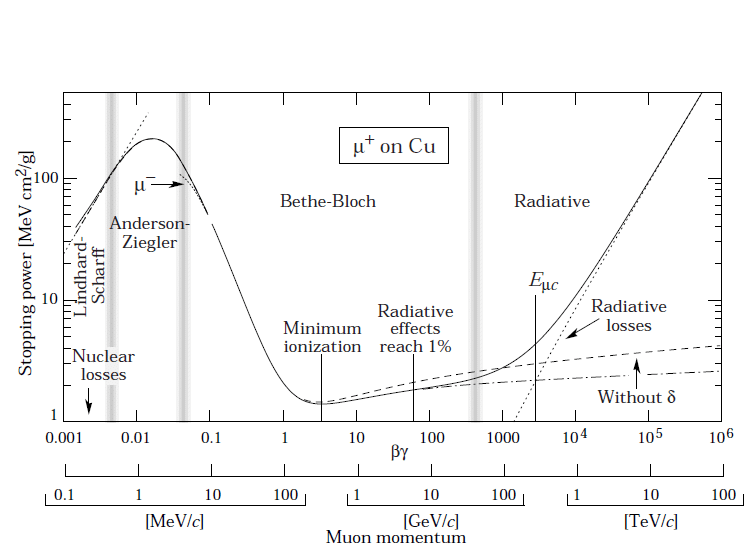
\includegraphics[scale=0.4]{Figures/The-Bethe-Bloch-forumula-for-positive-muons-in-copper-as-a-function-of-bg2-shown.png}
        \caption{Bethe Bloch graph.}
        \label{6}
\end{figure}

\begin{figure}[h!]
        \centering
        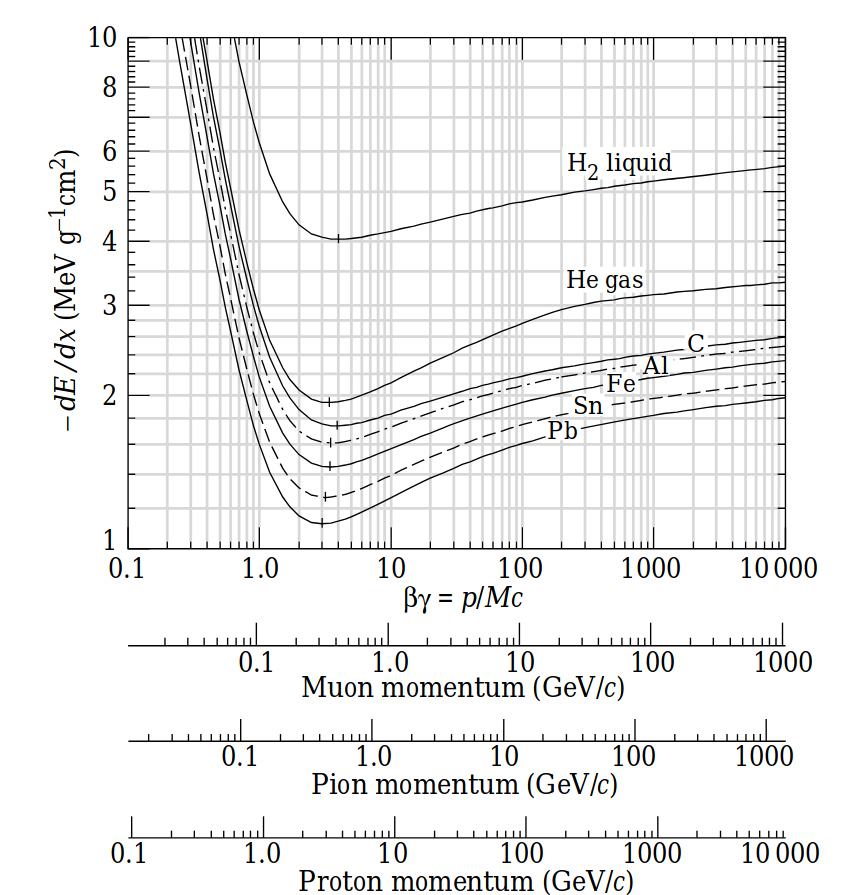
\includegraphics[scale=0.3]{Figures/bethe bloch medium.png}
        \caption{Bethe Bloch grap in different mediums.}
        \label{7}
\end{figure}

\newpage
\textbf{The Bragg Pea}k: because energy loss is inversely proportional to the square of the velocity ($1/\beta^2$), a heavy particle moving through matter exhibits a highly specific energy deposition profile known as the Bragg Curve. When entering the medium at high speed, the particle loses energy relatively slowly and uniformly. Right before the particle comes to a complete stop, its velocity drops drastically. This causes a massive, localized surge in energy deposition. Immediately after the peak, the particle runs out of kinetic energy and stops completely, dropping the energy deposition to zero. This phenomenon is the physical foundation for Proton Therapy in cancer treatment. Unlike conventional X-rays (photons), which deposit their maximum dose near the surface and damage healthy tissue all the way through the body, protons can be tuned to release their destructive peak dose directly inside a tumor, completely sparing the healthy tissue located behind it.

\begin{figure}[h!]
        \centering
        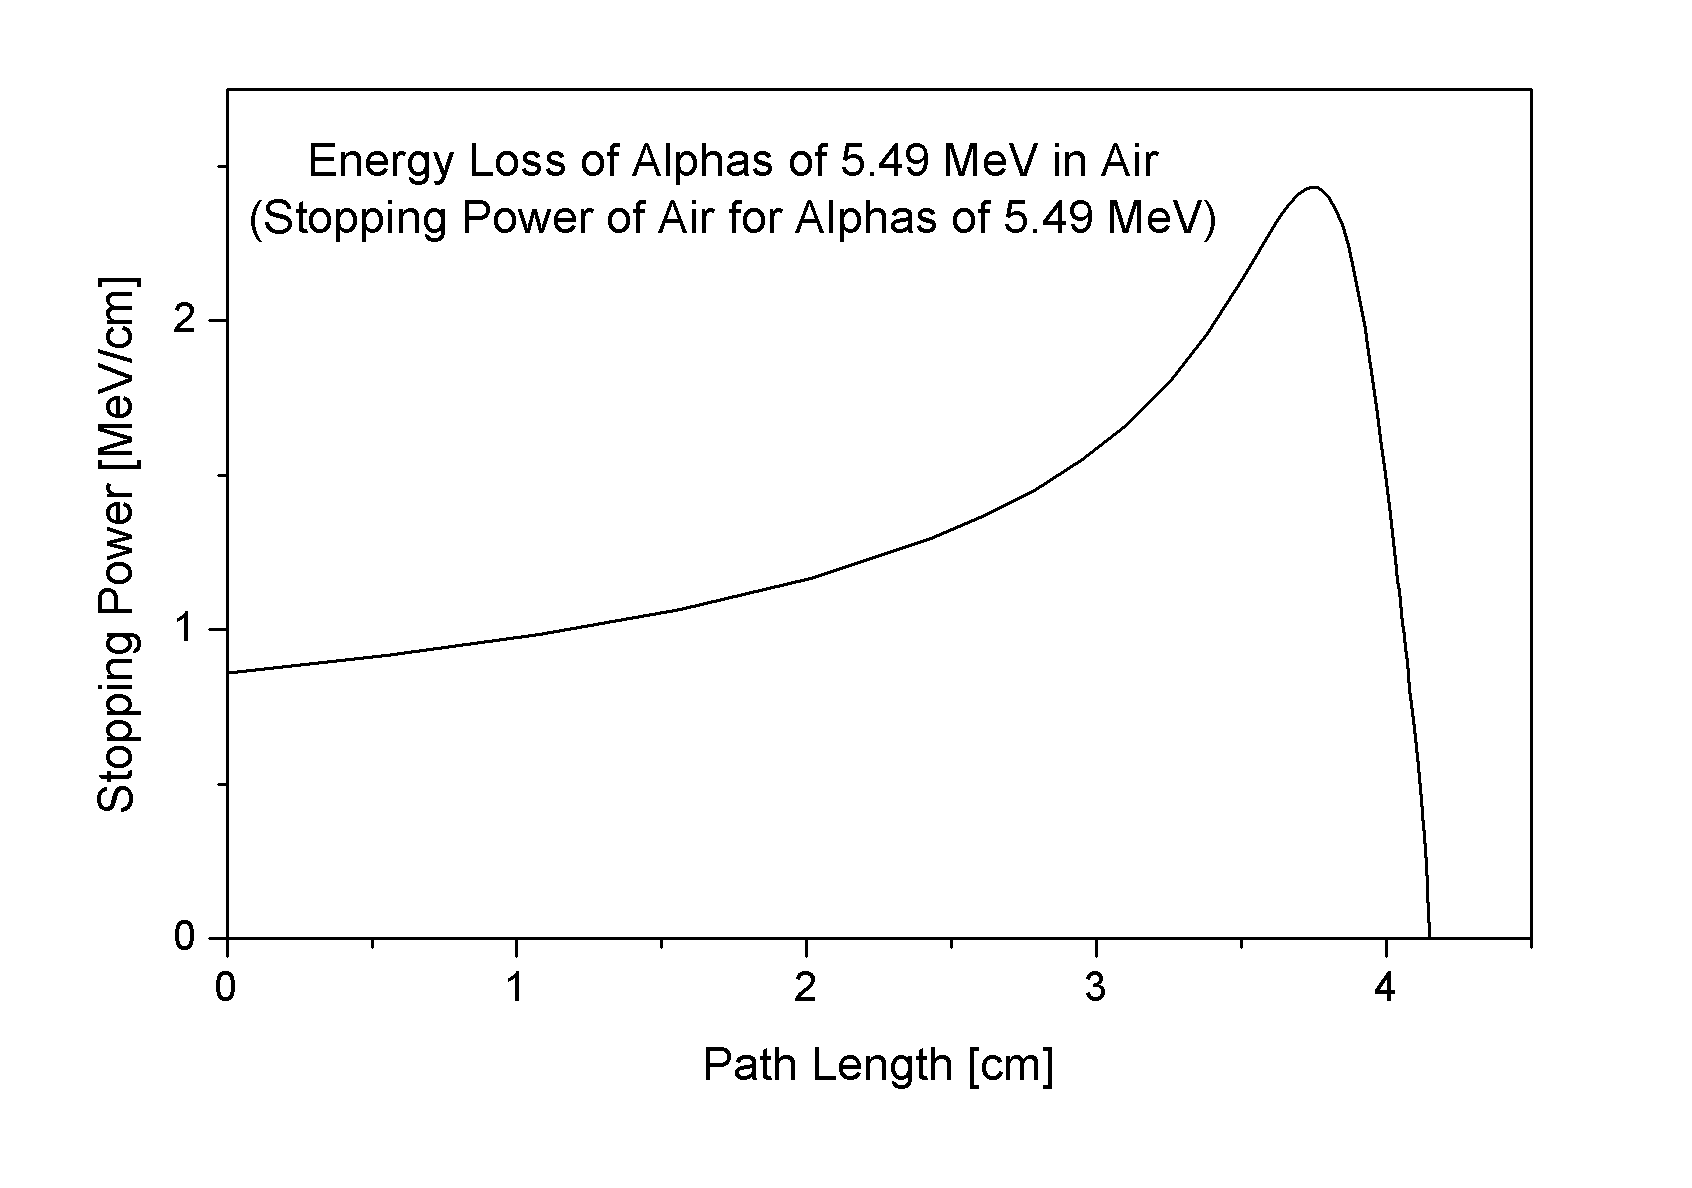
\includegraphics[scale=0.2]{Figures/bragg peak.png}
        \caption{Bragg peak.}
        \label{8}
\end{figure}

\textbf{Limitations}: where the Formula Breaks Down: the Bethe-Bloch formula is incredibly accurate, but it is not a universal law for all particles and energies. It fails under the following conditions: 

\textbf{Electrons and Positrons}: Because electrons are incredibly light, they experience massive deflections (not straight lines) and lose significant energy via Bremsstrahlung (deceleration radiation), which Bethe-Bloch does not account for.

\textbf{Ultra-High Energies}: At ultra-high energies, radiative losses (like nuclear interactions or Bremsstrahlung for heavy ions) begin to dominate over the electronic ionization described by Bethe-Bloch.

While the electronic (collisional) stopping power dominates at lower energies, radiative stopping power becomes the overwhelming driver of energy loss when light charged particles (specifically electrons and positrons) reach relativistic speeds. Radiative stopping power is the energy loss per unit distance due to the emission of electromagnetic radiation—specifically Bremsstrahlung—as the particle is accelerated or decelerated by the intense electric fields of target nuclei.

For a relativistic electron of energy $E$ moving through a medium with atomic number $Z$ and nuclear density $N$, the radiative stopping power can be approximated as:$$-\left(\frac{dE}{dx}\right)_{\text{rad}} = N \cdot E \cdot Z^2 \cdot \sigma_{\text{rad}}$$
Where:
\begin{itemize}
    \item  $\sigma_{\text{rad}}$ is the cross-section for Bremsstrahlung emission. From this relationship, we can extract three critical physical insights
    \item Linear Dependence on Energy ($E$): Unlike collisional loss (which decreases at high energies before flatlining), radiative loss increases linearly with the particle's energy. The more energetic the electron, the more violently it radiates when deflected.
    \item Quadratic Dependence on Atomic Number ($Z^2$): The deceleration depends heavily on the charge of the target nucleus ($Z$). An electron passing through Lead ($Z=82$) will experience a radiative stopping power roughly 100 times greater than an electron of the same energy passing through Oxygen ($Z=8$).
    \item Proportionality to Density ($N$): More nuclei per unit volume means more deflection opportunities.
\end{itemize}

Also, the radiated power scales as:  $$P \propto \left(\frac{1}{m}\right)^2$$ 
Because an electron is roughly 1,836 times lighter than a proton, its acceleration in the same electric field is nearly 2,000 times greater, making its radiated power roughly $3.4 \times 10^6$ times larger. This is why radiative stopping power is practically negligible for heavy particles (protons, alpha particles) but paramount for electrons and positrons






\section{Electron and positrons matter interaction}

When it comes to electrons and positrons, the clean, straight-line trajectory of the Bethe-Bloch formula goes out the window. Because electrons and positrons have a tiny mass ($m_e$), they behave completely differently than heavy charged particles like protons or alpha particles. Instead of plowing straight through a material, they get buffeted around wildly, losing energy through two entirely distinct mechanisms: collisional (ionization) losses and radiative (Bremsstrahlung) losses.1. The Two Channels of Energy LossThe total stopping power for light particles is the sum of two components:$$\left(\frac{dE}{dx}\right)_{\text{total}} = \left(\frac{dE}{dx}\right)_{\text{coll}} + \left(\frac{dE}{dx}\right)_{\text{rad}}$$A. Collisional Losses (Ionization and Excitation)At lower energies, electrons/positrons lose energy just like heavy particles—by kicking atomic electrons out of their shells. However, the mathematical description (the Bethe formula for electrons) has to be modified for two quantum mechanical reasons:Identical Particles: When an incident electron hits an atomic electron, they are completely indistinguishable. You cannot tell which one was the projectile and which was the target after the collision.Kinematics: Because the projectile and target have identical masses, a single collision can deflect the incident electron by a massive angle, transferring up to 100\% of its kinetic energy.B. Radiative Losses (Bremsstrahlung)As the electron’s velocity approaches the speed of light, a new mechanism dominates. When a high-speed electron passes close to a highly charged atomic nucleus, the intense electric field violently deflects and decelerates it.According to classical electrodynamics, any accelerating or decelerating charge must emit electromagnetic radiation. This deceleration radiation is called Bremsstrahlung (German for "braking radiation").  2. The Critical Energy ($E_c$)The ratio between radiative and collisional energy losses scales roughly with the electron's energy ($E$) and the atomic number ($Z$) of the material:$$\frac{(dE/dx)_{\text{rad}}}{(dE/dx)_{\text{coll}}} \approx \frac{E \cdot Z}{800 \text{ MeV}}$$This gives rise to the concept of Critical Energy ($E_c$), which is the exact energy at which radiative losses become equal to collisional losses.In heavy materials (like Lead, $Z=82$): $E_c$ is very low ($\approx 7 \text{ MeV}$). This means even moderately energetic electrons will mostly lose energy via Bremsstrahlung.In light materials (like Water/Tissue, $Z \approx 7.5$): $E_c$ is much higher ($\approx 80 \text{ MeV}$). In the human body, medical linear accelerators (usually operating under $25 \text{ MeV}$) utilize electrons that lose energy predominantly through ionization.  3. Trajectory and Depth-Dose ProfileBecause electrons are so light, their paths through matter are chaotic and zigzagged. They undergo severe multiple Coulomb scattering.  Unlike protons, which have a crisp Bragg Peak, electrons do not have a sharp ending point:No Bragg Peak: The continuous large-angle scattering smears out the energy deposition.Surface Dose: Electrons deposit a significant amount of energy right at the surface of the material.Range Straggling: If you shoot 100 electrons with the exact same energy into a material, they will all stop at vastly different depths because their randomized, zigzag paths vary so wildly.4. The Positron Twist: AnnihilationEverything stated above applies equally to both electrons and positrons. However, because the positron is antimatter, it has a unique finale once it slows down to thermal energies.Positronium Formation: Before dying, a slow positron often pairs up with a free electron to form an exotic, brief "atom" called positronium.Annihilation: Within nanoseconds, the electron and positron annihilate each other. Their masses are completely converted into pure energy, producing two gamma-ray photons, each with an energy of exactly $0.511 \text{ MeV}$ (the rest mass of an electron), shooting out at exactly $180^\circ$ apart to conserve momentum.

\begin{figure}[h!]
        \centering
        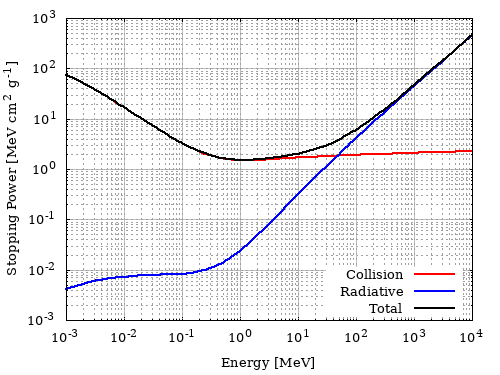
\includegraphics[scale=0.5]{Figures/electron positron stopping power.png}
        \caption{Electron stopping power.}
        \label{9}
\end{figure}

\section{Alpha decay}

Many heavy nuclei decay via $\alpha$ emission (a $^4$He
nucleus), in particular most of the nuclei with $A> 90$ are energetically unstable against $\alpha$ emission but only half of these actually emit. $$^{A}_{Z}\text{X} \longrightarrow ^{A-4}_{Z-2}\text{Y} + ^{4}_{2}\text{He} + Q$$
with $\text{X}$ Parent nucleus, $\text{Y}$ Daughter nucleus, $^{4}_{2}\text{He}$ The alpha particle and $Q$ The disintegration energy (the energy released during the decay, also called Q value). 
Alpha decay happens via quantum tunnelling through a barrier of potential. 

\begin{figure}[h!]
        \centering
        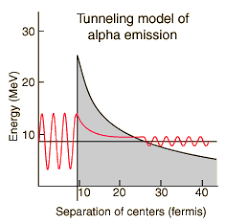
\includegraphics[scale=0.7]{Figures/quantum tunnel.png}
        \caption{$\alpha$ decay quantum tunnelling.}
        \label{10}
\end{figure}


The energetics of the process is the following: $$Q = \left( m_{\text{parent}} - m_{\text{daughter}} - m_{\alpha} \right) c^2$$

Because momentum must be conserved, the released energy is split between the two products. Since the daughter nucleus is much heavier than the alpha particle, the alpha particle carries away the vast majority of the kinetic energy (typically around $98\%$), shooting away at speeds up to $5\%$ the speed of light. 

The probability of tunneling is incredibly sensitive to the energy of the alpha particle. A small increase in the alpha particle's energy results in a massive increase in its chances of escaping.This relationship is described by the Geiger-Nuttall Law:$$\log_{10} T_{1/2} = \frac{A}{\sqrt{E}} + B$$Where $T_{1/2}$ is the half-life, $E$ is the kinetic energy of the alpha particle, and $A$ and $B$ are constants.Because of this square-root dependency, a tiny variation in decay energy spans astronomical differences in half-lives. For example: Polonium-212 emits an $8.9 \text{ MeV}$ alpha particle and has a half-life of $0.3$ microseconds. Uranium-238 emits a $4.3 \text{ MeV}$ alpha particle and has a half-life of $4.5$ billion years.

\begin{figure}[h!]
        \centering
        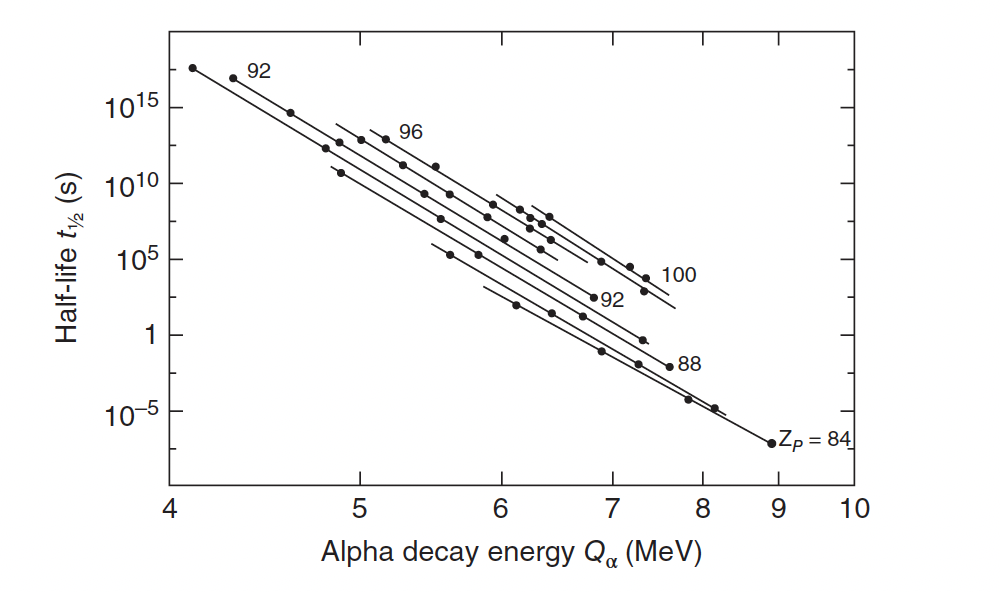
\includegraphics[scale=0.5]{Figures/geiger nuttal.png}
        \caption{$\alpha$ decay quantum tunnelling.}
        \label{11}
\end{figure}

\section{Beta decay}

Beta decay is a type of radioactive decay in which an unstable atomic nucleus transforms into a more stable one by altering its proton-to-neutron ratio. This process is mediated by the weak nuclear force and results in the emission of beta particles (highly energetic electrons or positrons). Here is a breakdown of the general features, types, and fundamental principles of beta decay.1. The Two Main Types of Beta Decay

\textbf{Beta decay} occurs in two primary ways, depending on whether the nucleus has too many neutrons or too many protons.  \\
\textbf{Beta-Minus Decay} ($\beta^-$). 
When it happens: Occurs in neutron-rich nuclei.  The Process: A neutron inside the nucleus converts into a proton. To conserve charge and lepton number, the nucleus emits an electron (the $\beta^-$ particle) and an electron antineutrino ($\bar{\nu}_e$).  Nuclear Equation:$$n \rightarrow p + e^- + \bar{\nu}_e$$Result: The atomic number ($Z$) increases by 1, but the mass number ($A$) remains the same. Example: Carbon-14 decays into Nitrogen-14.  $$^{14}_{6}\text{C} \rightarrow ^{14}_{7}\text{N} + e^- + \bar{\nu}_e$$

\textbf{Beta-Plus Decay ($\beta^+$) / Positron Emission}.
When it happens: Occurs in proton-rich nuclei.  The Process: A proton inside the nucleus converts into a neutron. To maintain balance, the nucleus emits a positron (the $\beta^+$ particle, which is the electron's antiparticle) and an electron neutrino ($\nu_e$).  Nuclear Equation:$$p \rightarrow n + e^+ + \nu_e$$Result: The atomic number ($Z$) decreases by 1, while the mass number ($A$) stays the same.Example: Carbon-11 decays into Boron-11.  $$^{11}_{6}\text{C} \rightarrow ^{11}_{5}\text{B} + e^+ + \nu_e$$.

\begin{figure}[h!]
        \centering
        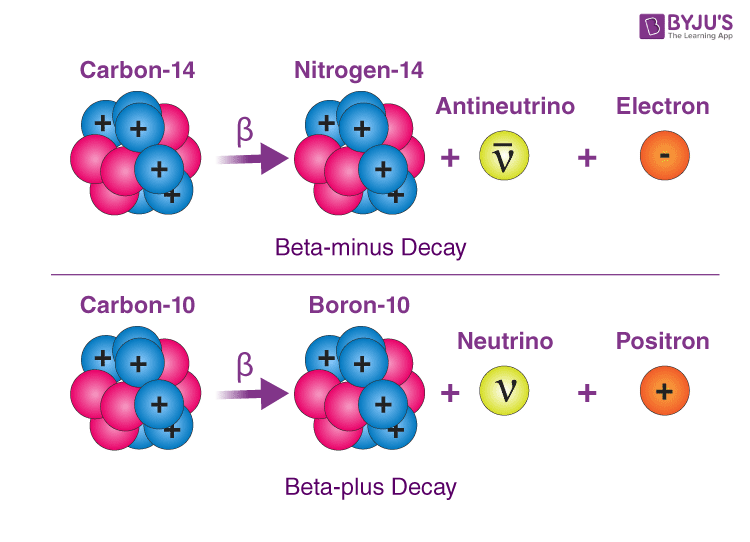
\includegraphics[scale=0.3]{Figures/beta decay.png}
        \caption{$\beta$ decay.}
        \label{12}
\end{figure}


The Continuous Energy Spectrum (and the Neutrino's Discovery)Unlike alpha decay, where particles are ejected with discrete, specific energies, beta particles are emitted with a continuous spectrum of kinetic energies.  For a long time, this baffled physicists because it looked like energy was disappearing. In 1930, Wolfgang Pauli proposed that a third, virtually invisible particle was sharing the energy—the neutrino. Because the energy is split randomly between the beta particle and the neutrino, the beta particle can exit with anything from zero energy up to a maximum threshold ($E_{\text{max}}$). Beta decay strictly obeys several fundamental laws of physics:Conservation of Charge: Total electric charge before and after the decay remains identical. Conservation of Nucleon Number: The total number of protons and neutrons ($A$) does not change.  Conservation of Lepton Number: Electrons and neutrinos are leptons. In $\beta^-$ decay, a lepton ($e^-$) and an anti-lepton ($\bar{\nu}_e$) are created, keeping the net lepton number change at zero.  Penetration and Hazard LevelBeta particles are much smaller and lighter than alpha particles, meaning they travel faster and are more penetrating. They can travel a few meters in the air and penetrate a few millimeters of human skin or aluminum.  While they pose an internal hazard if ingested or inhaled, they can be effectively shielded by a thin sheet of plastic, glass, or aluminum.

\textbf{Electron Capture (EC)}.
Often grouped with beta decay, electron capture is a competing process for proton-rich nuclei. Instead of emitting a positron, the nucleus "captures" an inner-shell electron (usually from the K or L shell).The captured electron combines with a proton to form a neutron and emits a neutrino:$$p + e^- \rightarrow n + \nu_e$$Like $\beta^+$ decay, the atomic number decreases by 1, and the mass number remains unchanged.

\begin{figure}[h!]
        \centering
        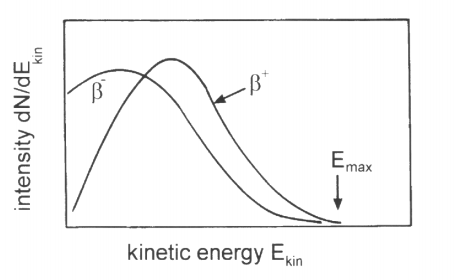
\includegraphics[scale=0.8]{Figures/beta deacy spectrum.png}
        \caption{$\beta$ decay spectrum.}
        \label{13}
\end{figure}

\end{document}